\begin{surferPage}[A1+- Singularity]{$A^{+-}_1$--Singularity (Double Cone)}
    The double cone (also called ordinary double point or singularity of type $A_1^{+-}$) is the
    simplest singularity:
    when deforming the equation
    \[x^2+y^2-z^2=0\]
    slightly, it becomes smooth.
    The pictures below show surfaces corresponding to the equation
    \[x^2+y^2-z^2=a\]
    for the values $a=-\frac12$, $a=0$, $a=\frac12$:
    %
    \begin{center}
      \vspace*{-0.4em}
      \begin{tabular}{@{}c@{\quad}c@{\quad}c@{}}
        \begin{tabular}{@{}c@{}}
          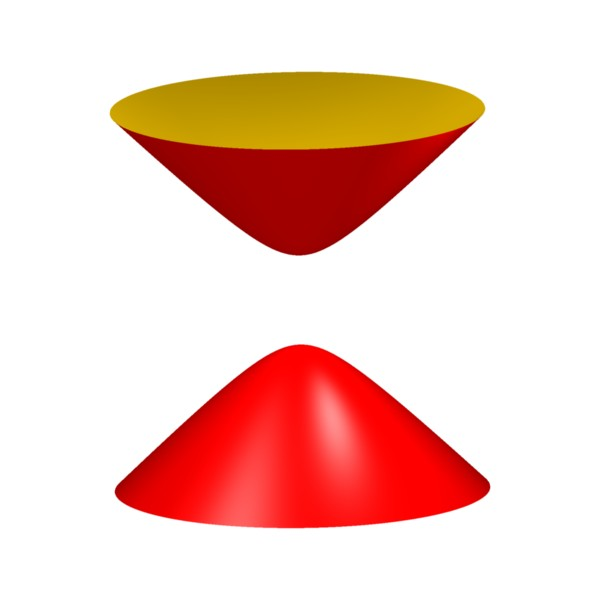
\includegraphics[width=1.2cm]{../../common/images/A1pm_0}
        \end{tabular}
        &
        \begin{tabular}{@{}c@{}}
          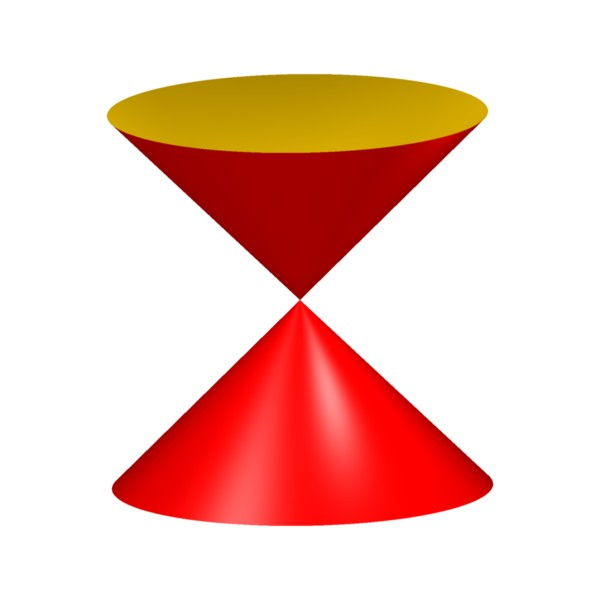
\includegraphics[width=1.2cm]{../../common/images/A1pm_1}
        \end{tabular}
        &
        \begin{tabular}{@{}c@{}}
          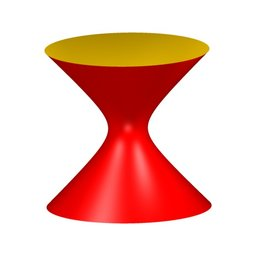
\includegraphics[width=1.2cm]{../../common/images/A1pm_2}
        \end{tabular}
      \end{tabular}
    \end{center}
    \vspace*{-0.4em}
    For negative $a$ the deformation is a hyperboloid of two sheets and for positive $a$ it is a connected hyperboloid of one sheet.

    We will see in the following examples that it is possible to deform more
    complicated singularities in a way such that several double cones develop. Each of them can then be deformed into a one- or two--sheeted hyperboloid.
\end{surferPage}
